% introduction.tex



% TODO: eventuell alle 'x86' in amd64 umbenennen, und 'ARM' in arm64




\section{Introduction}


% 2. Absatz: Lösungsvorschlag in diesem Paper und dann kommt das Goal
% letzter Absatz der Introduction: 
%       The remainder of this paper is structured as follows: In section II, we ...
The use of processors with Arm Big Little technology has already shown a possible reduction in power consumption of operating a device with heterogeneous Central Processing Unit (CPU) cores.
Processors that use ARM Big Little architectures have both performance and efficiency cores, 
between which processes are distributed for maximum efficiency
which leads to the lower energy consumption of the device.

%The goal of this paper is to scale this idea up for potential use in data centers.
Instead of integrating two different types of cores into one processor, the idea is to build a heterogeneous cluster with different CPU architectures to achieve the same effect.
%The term heterogeneous in this context refers to the two types of processor architectures, which are used within a cluster. 
% TODO: Klaus' Experiment einleiten.



%For the prototype cluster proposed in this paper, 
%the container orchestration technology Kubernetes 
%\cite{kubernetesIo} is used.
%The results are used to propose a guideline for running container workloads
%in a heterogeneous environment with machines of different processor architectures.

%For the prototype cluster proposed in this paper, 
%we will make use of
%the container orchestration technology
%Kubernetes \cite{kubernetesIo}
%and propose a guideline for running container workloads
%in a heterogeneous environment with
%machines of different processor architectures.

 

% Igor: Vor allem...das große Ziel wäre, dass die Introduction genau eine Seite Lang ist und auf Seite 1 aufhört


The use of containers offers many advantages when it comes to running applications. 
They allow a high degree of independence from the base system and still offer a lower performance overhead than virtual machines. 
However, since they are also a form of virtualization, they are not independent of the processor architecture and must be adapted for each type of processor architecture. 
This is one of the problems that limit the cross-platform use of containers. 
With traditional software operations, it was often very difficult to move application deployments from one to another completely different system. The use of cloud technologies and especially containers can make this easier to implement. 
Individual containers can be moved between physical or virtual machines by container orchestration software.
At the same time their computing power can be combined by using load balancing techniques.
%The self-contained independent nature of containers also allows for migration between cloud service providers almost seamlessly.


%Lowering energy consumption by using heterogeneous clusters
Different processor architectures also provide advantages in certain tasks and their performance can also be tailored to specific applications.
This could be used as a smart and energy-efficient way of load balancing and to reduce the energy consumption of the running applications. 
As a result, operations can be made more efficient and operating costs can be lowered. 
To answer this question, this paper will compare two processor architectures and determine their energy efficiency in specific tasks.
%To reduce complexity, only two types of application will be used for the test later in the paper. 
%A large number of different applications with different hardware omissions significantly increases the complexity of the experiment and also makes it more difficult to determine the benefits of energy-efficient load balancing.



%Benefits of heterogeneous clusters for data centers
A useful application for saving energy by using heterogeneous clusters efficiently are data centers.
By reducing the energy used to operate the server infrastructure, the active operating costs for the server hardware can be lowered. 
However, the reduced energy consumption also creates other benefits. 
Much of the energy consumed by computers is converted into heat, which in the case of a data center requires a cooling system. 
With a reduction in energy consumption and a higher energy efficiency, the required cooling capacity for the overall system also decreases. 
This in turn also reduces the required amount of cooling and thus also physical space in the data center.
This can result in twice the energy saving as energy can be saved for both the operation and the cooling of the system at the same time.
By using a cluster with heterogeneous CPU architectures, the efficiency of older hardware can also be increased by adding some newer systems.
Older hardware usually has a significantly lower performance per watt than modern hardware.
For that reason the application with the highest difference in energy efficiency should be run on the new hardware.

%Distribution of consumed energy in datacenters
In a report from \citeauthor{shehabi2016united}, the data shows that servers, 
as well as cooling and power provision systems each make up 43 \% of U.S. data center electricity use, 
which together are 86 \%. 
Other minor contributors are storage with 11 \% and networking with 3 \%.
(see Figure \ref{fig:electricityUseDatacenter2014})
\cite{shehabi2016united}.

%Piechart
\begin{figure}[h]
	\centering
	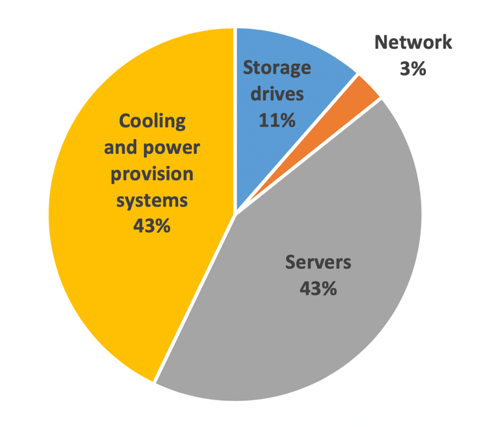
\includegraphics[width=.55\linewidth]{fig/electricityUseDatacenter2014.png}
	\caption{Fraction of U.S. data center electricity use in 2014, by end use
	    (\citeauthor{shehabi2016united}, \citeyear{shehabi2016united}).
	}
	\label{fig:electricityUseDatacenter2014}	
\end{figure}